\documentclass[12pt]{article}
\usepackage{geometry} 
\geometry{a4paper}
\usepackage{listings}
\usepackage[utf8]{inputenc}
\usepackage{listings}
\usepackage{xcolor}
\usepackage{graphicx}
\usepackage{float}
\usepackage{caption}
\usepackage{subcaption}
\usepackage{amsmath}
\usepackage{algorithm}
\usepackage[noend]{algpseudocode}
\usepackage[shortlabels]{enumitem}
\usepackage[overload]{empheq}
\usepackage{url,apacite}    % package url to prevent horrible linebreaks
\bibliographystyle{apacite}

\definecolor{codegreen}{rgb}{0,0.6,0}
\definecolor{codegray}{rgb}{0.5,0.5,0.5}
\definecolor{codepurple}{rgb}{0.58,0,0.82}
\definecolor{backcolour}{rgb}{0.95,0.95,0.92}
\lstdefinestyle{mystyle}{
	backgroundcolor=\color{backcolour},   
	commentstyle=\color{codegreen},
	keywordstyle=\color{magenta},
	numberstyle=\tiny\color{codegray},
	stringstyle=\color{codepurple},
	basicstyle=\ttfamily\footnotesize,
	breakatwhitespace=false,         
	breaklines=true,                 
	captionpos=b,                    
	keepspaces=true,                 
	numbers=left,                    
	numbersep=5pt,                  
	showspaces=false,                
	showstringspaces=false,
	showtabs=false,                  
	tabsize=2
}
\lstset{style=mystyle}

\title{Programming project}
\author{Umberto Cocca}
\date{} 

\begin{document}
\maketitle
\noindent \textbf{The Problem}\\
Let R be an axis-parallel rectangle and $D = \{d_1, ..., d_n\}$ a collection of closed circular disks.
Each disk $d_i$ is represented by its center $p_i$, which lies within $R$, and its positive radius $r_i$. Disks may extend outside of $R$, and one disk may be contained within another.

\begin{itemize}
	\item If every point of $R$ lies within at most one disk of $D$ then we say that the
	elements of $D$ form a packing of $R$ . Implement a plane-sweep $O(n log n)$ time algorithm
	that determines whether $D$ is a packing of $R$
	\item If every point of $R$ lies within at least one disk of $D$ then we say that the elements of $D$ form a cover of $R$. Implement a plane-sweep $O((n+m) log n)$ time algorithm that determines whether $D$ is a cover of $R$, where m is the number of intersection points lying within $R$ between the boundaries of disks. The running time should not depend on
	the number of intersection points that lie outside of $R$.
\end{itemize}


\noindent \textbf{Solution}\\
For the first problem if I proof that exists at least an intersection between two circles then the elements of $D$ do not form a packing of $R$. \\

\noindent For the second problem if I proof that exists at least one intersection h where h is not within any circule then we can state that the elements of $D$ do not form a cover of $R$. \\

\noindent \textbf{Implementation}\\
The programming language used is Python with the following main modules:
\begin{itemize}
	\item cv2: visual presentation to project the points in 2d image and look at what happens at each iteration
	\item numpy: used especially for some tasks during the animation
	\item pdb: it is debugger for python
	\item math: to execute specific calculations
\end{itemize}

\noindent First of all, was parsed the input file, which has the minimum and maximum x-coordinate in its first line: $x_{min}$ $x_{max}$ and the respective coordinates for the y-coordinate in the second line: $y_{min}$ $y_{max}$. Each following line descrives a circle with center $c=(c_x, c_y)$ and radius $r$ by: $c_x$ $c_y$ $r$. Thus, the function $parseInput()$ returns the max coordinate $x$, $y$ and an list of $circles$ object. After, the $draw(x,y,circles)$ is a function that computes all the intersection among all the circles and plot this information above the circles. The unique intention about this function is only to have a visual representation of the input at the beginning.

\begin{figure}[H]
	\centering
	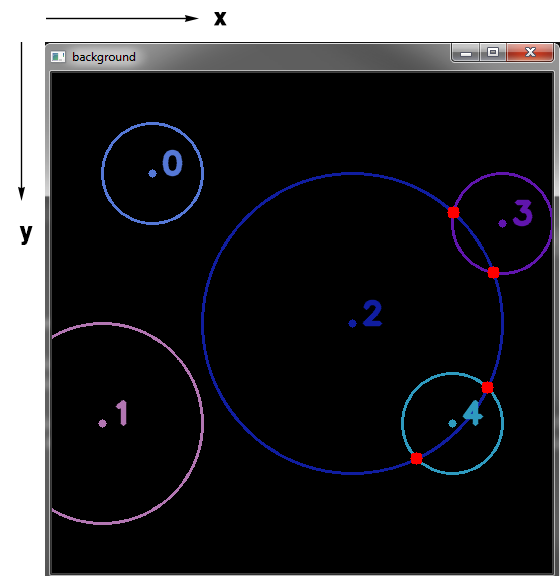
\includegraphics[scale=0.45]{img/1.png}
	\caption{Plane sweep screenshot captured with the $draw()$ function. There are 5 circles in the scene and 4 red points that represent the intersections among all the circles.} \label{fig:1b}
\end{figure}

\noindent It is important notice that the origin is on top left of the picture and the orientation is positive from left to right and from top to down. Therefore, the circle $1$ has coordinate $x=1, y=7$ and it is "above" the circle $0$. Likewise, the circle $0$ is "below" the circle $1$. Afterwards, was effectively implemented the first plane sweep algorithm to identify if all the elements of $D$ form (or not) a packing of $R$. The function is called $planeSweepPacking(x, y, circles, animation = False)$, where $x$ and $y$ are the dimensions of the rectangle $R$, circles is the list of all circles in input and finally animation is a boolean that if it is set $True$ permits to look at the algorithm step by step for each event in the event queue, otherwise if $False$ runs all the algorithm without stops. Inside the function a dictionary of events, named "eventsQueue" is created. For each circle 2 events are generated: "LEFT" and "RIGHT", where for "LEFT" the point event is given by $c_x$ point - $radius$, while the "RIGHT" event is given by $c_x$ point + $radius$. All the events are ordered by the point event, that is ordered by $x$ axis.  

\begin{lstlisting}
eventsQueue = {
	"event1" : {
		"obj" : event1,
		"before" : "event0",
		"after" : "event2",
	},
	
	"event2" :{
		"obj" : event2,
		"before" : "event1",
		"after" : "event3",
	}
}
\end{lstlisting}

\noindent Above there is an example of the "eventsQueue". For each element eventsQueue there are 3 properties: "obj", "before" and "after", where the first one points to the actual event, "before" is the string name of the event $i-1$ before the current event $i$ and similarly "after" is the string name of the event $i+1$ after the current event $i$. A dictionary for the sweepline was created as well:

\begin{lstlisting}
sweepline = {
	0 : {             # name of this circle
		"up" : None,    # name of the upper circle
		"me" : 0,       # name of this circle
		"below" : 2,    # name of the lower circle
	},
	
	2 :{
		"up" : 0,
		"me" : 2,
		"below" : 1,
	}
	
	1 :{
		"up" : 2,
		"me" : 1,
		"below" : None,
	}
}
\end{lstlisting}
Above there is an example of the "sweepline". For each element of the sweepline there are three properties: "up", "me" and "below", where "up" is the index of the circle above that circle $i$, "me" is the current circle $i$ and finally "below" is the index of the circle below that circle $i$. \\

\noindent Then, in order of priority, it is extracted from the eventsQueue an event and some actions are done related of the type of the event. If it is a "LEFT" event, but the point that represents it is out the rectangle, then the event is ignored, otherwise the sweepline is updated adding the new circle. If it is a "RIGHT" event, but the point that represents it is out of the rectangle, then the event is ignored, otherwise the sweepline is updated deleting the circle related to this event. Every time an event is extracted from the eventsQueue it is computed the intersection between the circle above and the circle related to the event and the intersection between the circle below and the circle related to this event. If an intersection is within the rectangle shape then it is reported that "the elements of $D$ do not form a packing of $R$", otherwise if no intersection detected for every event in the eventsQueue then it is stated that "the elements of $D$ form a packing of $R$". \\

\noindent Similarly, for the second plane sweep algorithm the function that it is called is $planeSweepCover(x, y, circles, animation)$ that has the same input. Even here, the eventsQueue and the sweepline are initialized in the same way as the alogorithm before. What changes are the action of the  events. In fact for each event is computed the intersections and these are added in a dictionary called $allIntersectionNotChecked$. At the end of every event, it is checked for every point intersection in allIntersectionNotChecked if it is within a circle in the sweepline. In conclusion, if there are still some points in allIntersectionNotChecked then it is reported "the elements of $D$ do not form a cover of $R$", otherwise "the elements of $D$ form a cover of $R$". \\


\noindent \textbf{Time complexity}\\
The average case times listed for dict objects assume that the hash function for the objects is sufficiently robust to make collisions uncommon. The average case assumes the keys used in parameters are selected uniformly at random from the set of all keys. \cite{wiki:xx1}

\begin{figure}[H]
	\centering
	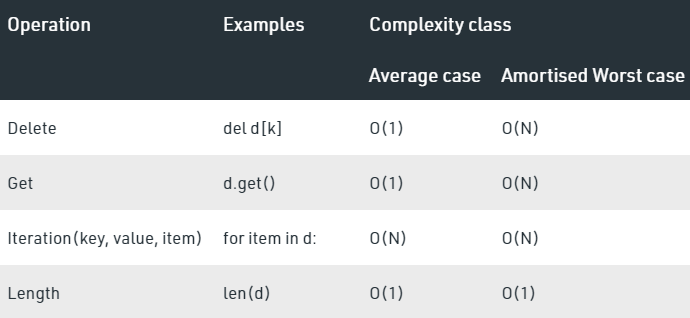
\includegraphics[scale=0.4]{img/2.png}
	\caption{Time complexity of dictionary in python of the operation used to implement the algorithms.} \label{fig:1b}
\end{figure}
\noindent The motivation for amortized analysis is that looking at the worst-case run time per operation, rather than per algorithm, can be too pessimistic. While certain operations for a given algorithm may have a significant cost in resources, other operations may not be as costly. The amortized analysis considers both the costly and less costly operations together over the whole series of operations of the algorithm. This may include accounting for different types of input, length of the input, and other factors that affect its performance \cite{wiki:xxx}. \\

\noindent Speaking about the total running time for the first problem there is the sort operation that requires $O(nlogn)$, then there are $n$ central points, in consequence left and right endpoints that is $2n$ events. With a dictionary each access takes $O(n)$ time at operation in the amortised worst case, hence the total time is $O(nlogn + 2n^2) = O(n^2)$ in the amortised worst case, while in the average case the delete and get operations require $O(1)$ time at each access and there is a $O(n)$ time for the iteration operation in total. Therefore, $O(nlogn + 2n)+O(n) = O(nlogn)$ as time complexity in the average case. \\

\noindent About the second algorithm there is the sort operation that requires $O(nlogn)$, then there are $2n + m$ events processed, where $n$ is the number of circles and $m$ are the number of intersections. Each event involves a constant amount of work and a constant number of accesses to the data structure that as mentioned in the first problem takes $O(n)$ time in the amortised worst case. Therefore, the total running time is $O(nlogn + (2n + m) n) = O(n^2 + mn) = O((n + m)n)$ time in the amortised worst case, while in the average case the delete and get operations require $O(1)$ time at each access and there is a $O(n)$ time for the iteration operation in total. Therefore, $O(nlogn + 2n+m)+O(n) = O(nlogn+m)$ as time complexity in the average case.

\noindent \textbf{Space complexity}\\
For the first problem the sweepline data structure contains at most one circle for each of the $n$ circles in the problem, so it is $O(n)$. In the eventsQueue points data structure, there can be $n$ starting points and $n$ end points $O(2n) = O(n)$. After one single intersection this forces the end of the program, hence eventsQueue is $O(1)$ and consequently the algorithm has $O(n)$ space complexity. \\

\noindent Speaking about the second problem the sweepline data structure contains at most one circle for each of the $n$ circles in the problem, so it is $O(n)$. In the eventsQueue points data structure, there can be $n$ starting points and $n$ end points $O(2n) = O(n)$. In addition, because only adjacent circles can have intersection points, there can be at most $2(n - 1)$ intersection points. Thus, eventsQueue should be $O(n)$ and therefore the algorithm should have $O(n)$ space complexity, but if the intersection points are saved related for each circles $O(n^2)$ this premits to exit from the algorithm in the middle of the program execution because it is possibile immediately report that the elements of $D$ do not form a cover of $R$ if a point intersection that belong at one circle $c_i$ is still in the allIntersectionNotChecked data structure and $c_i$ is deleted from the sweepline. For that reason, this implementation has $O(n^2)$. \\

\noindent \textbf{How to execute the code}\\
There is one file called main.py and different examples of input that must be in the same folder when it is runned the script. In the main function, to switch among the different inputs is enough to choose the file1 variable and comment the others called in the same way. It is foundamental comment the planeSweepCover statement to run the planeSweepPacking function, likewise comment planeSweepPacking to run the planeSweepCover function. To enable the animation it is enough simply set animation=True in planeSweepPacking or planeSweepCover functions, otherwise if not animation needed set animation=False.

\bibliography{wiki}
\end{document}